%doc: Revista 3/Res Llibres/ressenyes llibres.docx
\begin{news}
{2} %columnes
{Ressenyes de Llibres}
{}
{Fem Escola}
{03} %pagesof



\subsection*{La Castanyera}

\noindent\fbox{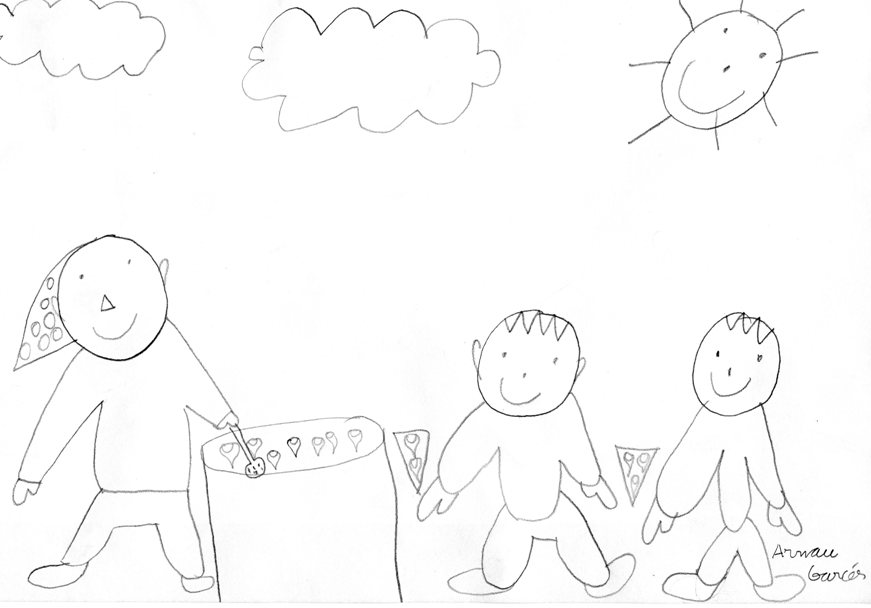
\includegraphics[width=7.5cm,keepaspectratio]{fem_escola/img/ressenya_img002.jpg}}

\emph{Autor: Anna Grau.  Editorial: Combel}

Una castanyera era molt amable, tant, que als nens que no portaven diners els donava castanyes i els deia que portessin els diners un altre dia. Però una altra castanyera, que era dolenta, com que no li compraven castanyes, va pensar robar les castanyes a l’altra. Llavors els nens li van donar castanyes a la castanyera amable, perquè en pogués continuar venent. Al final les dues es van fer amigues i van vendre juntes.

Aquest conte m’ha agradat perquè tracta de l’ amistat.

\authorandplace{Arnau Garcés}{1r de Primària}

\newpage

\subsection*{Els dos núvols amics}
\emph{Autor: Enric Larreula Editorial: Teide }

\noindent\fbox{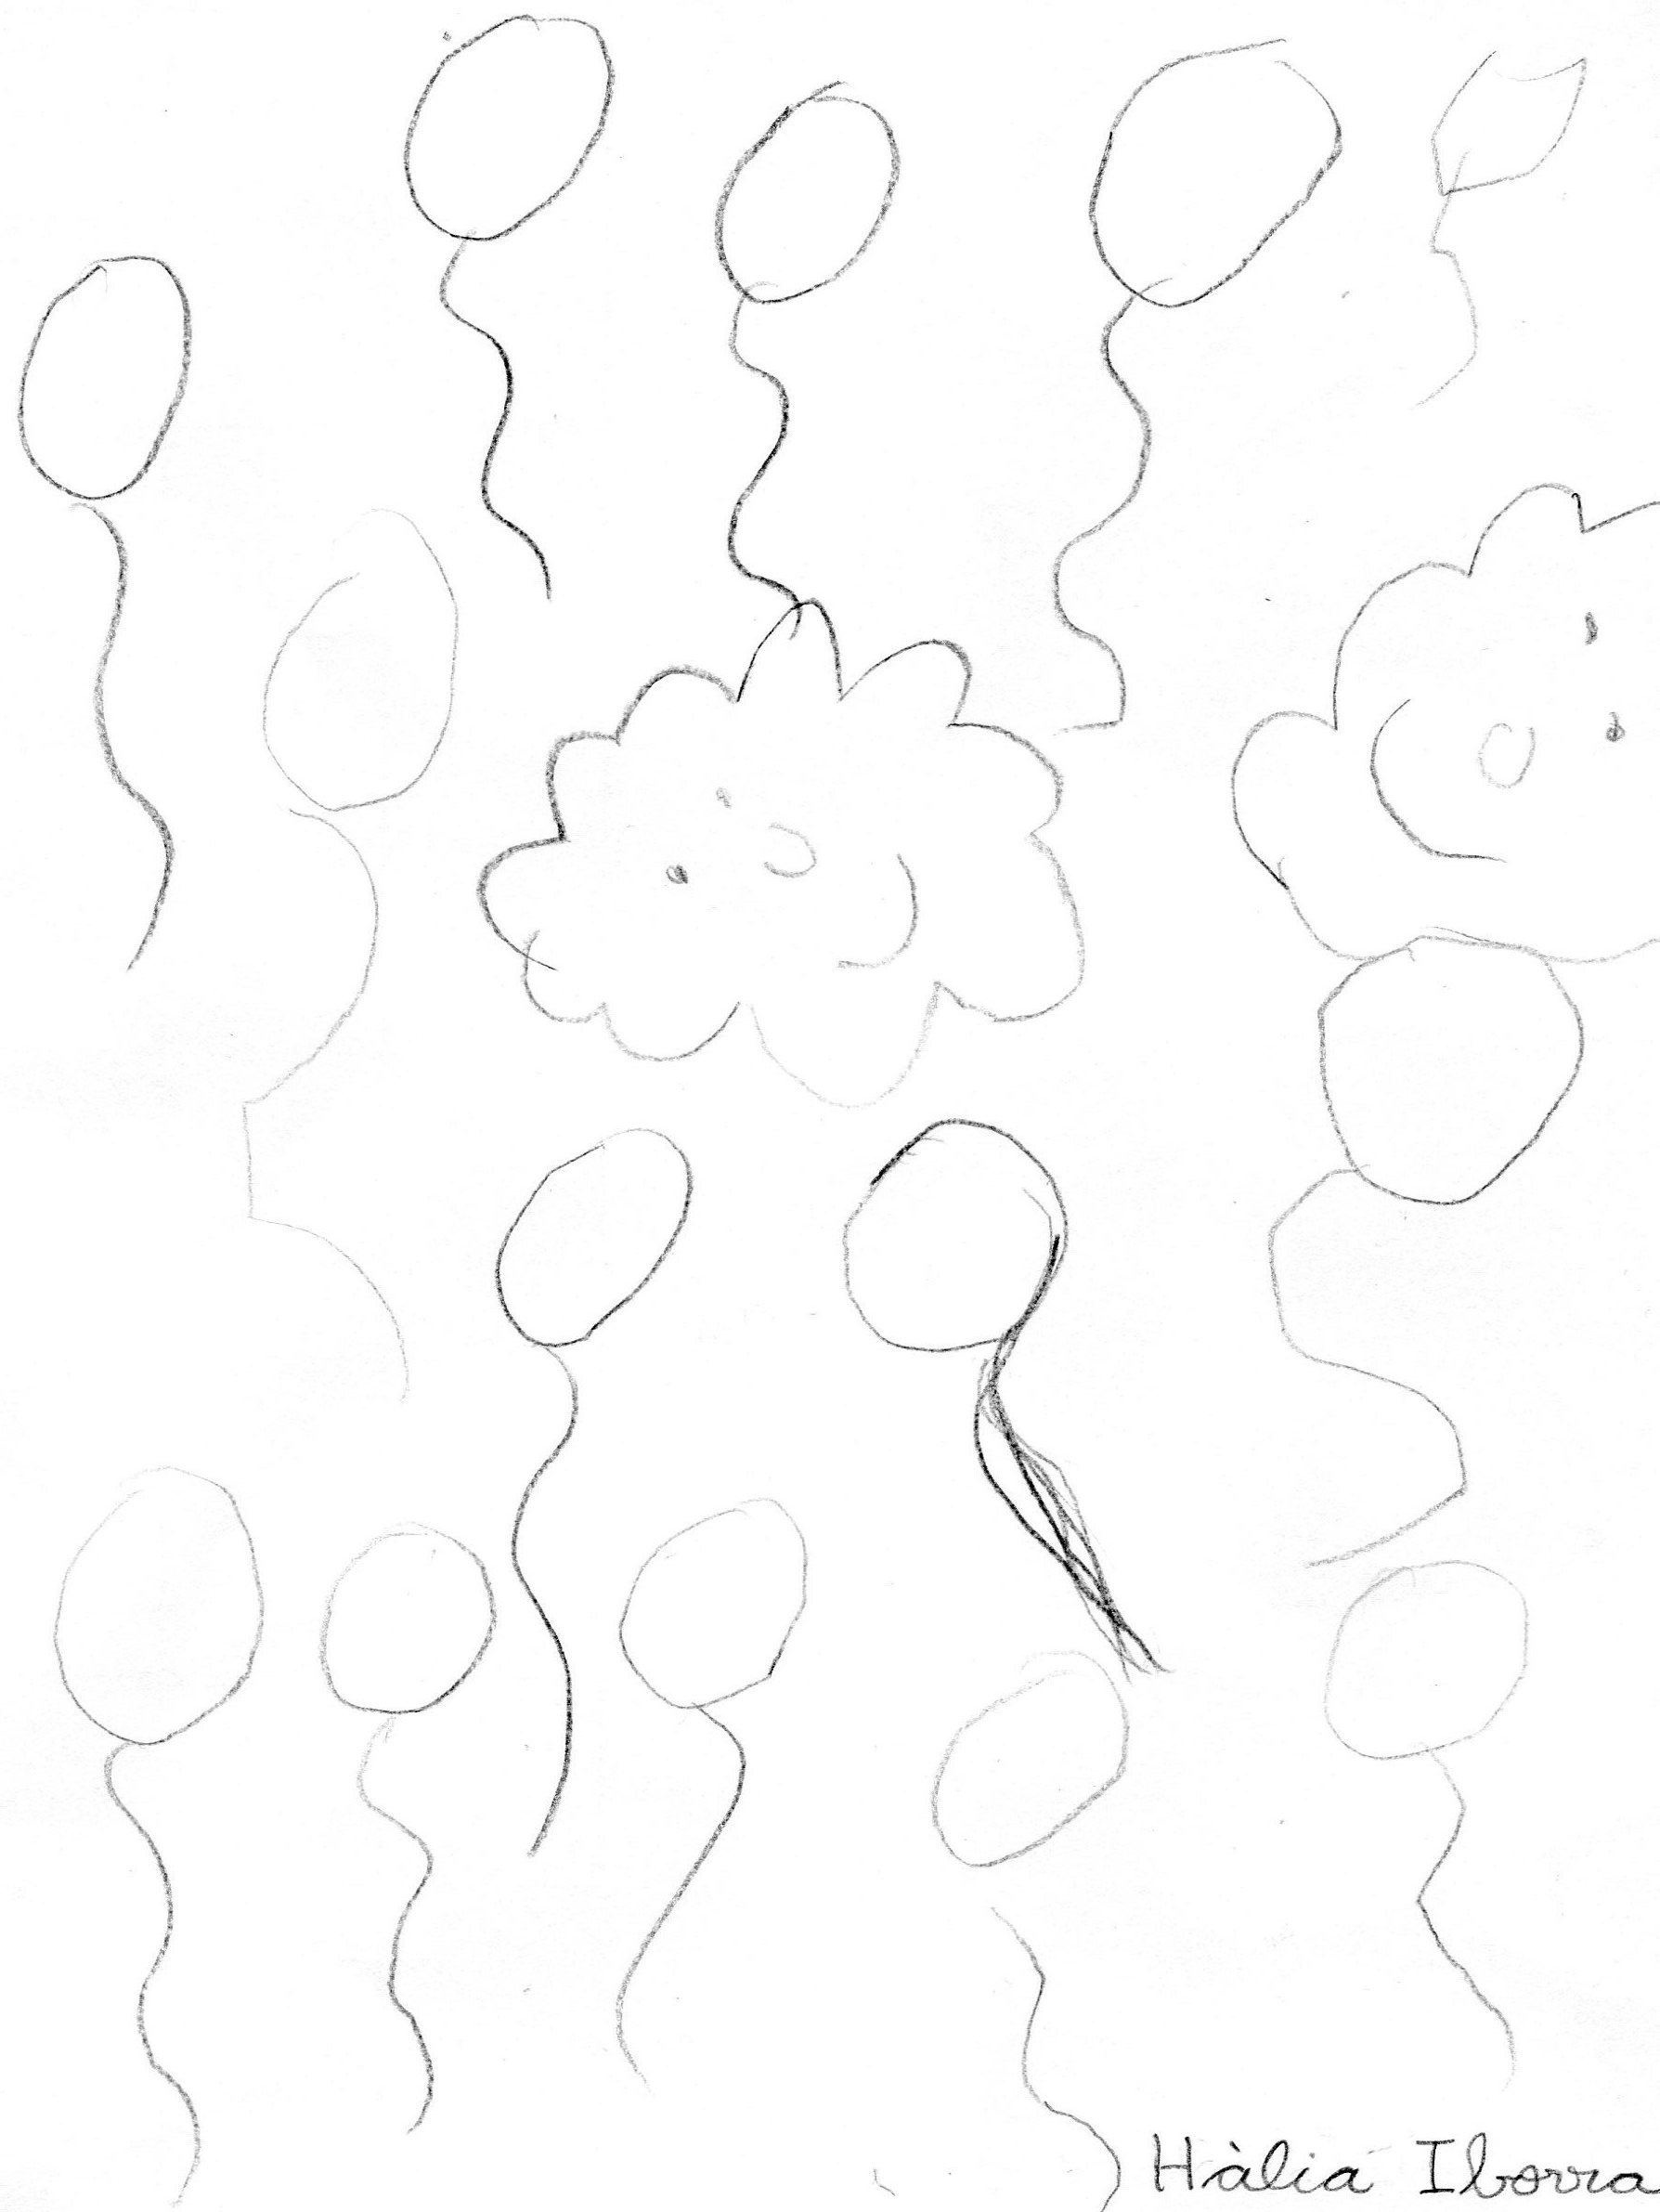
\includegraphics[width=5cm,keepaspectratio]{fem_escola/img/ressenya_img004.jpg}}

Els núvols són molt amics, viatjaven pel temps perquè els agradava estar molt junts. Un núvol estava amb els ocells i els altres estaven solets, els tiraven globus i un dia van caure a terra. Els agradava estar a les muntanyes, a vegades canviaven els colors: un era rosa i l’altre era lila. Un dia va fer molt vent i es van separar una mica, es va posar molt negre el cel i va ploure. Més tard va sortir el sol i els núvols van quedar enterrats.

He triat aquest llibre per l’amistat que demostren entre ells, pels jocs, pels viatges,...

\authorandplace{Hàlia Iborra}{1r de Primària}

\subsection*{La història de l’Ernest}
\emph{Autor: Mercè Company   Editorial: Cruïlla}


\noindent\fbox{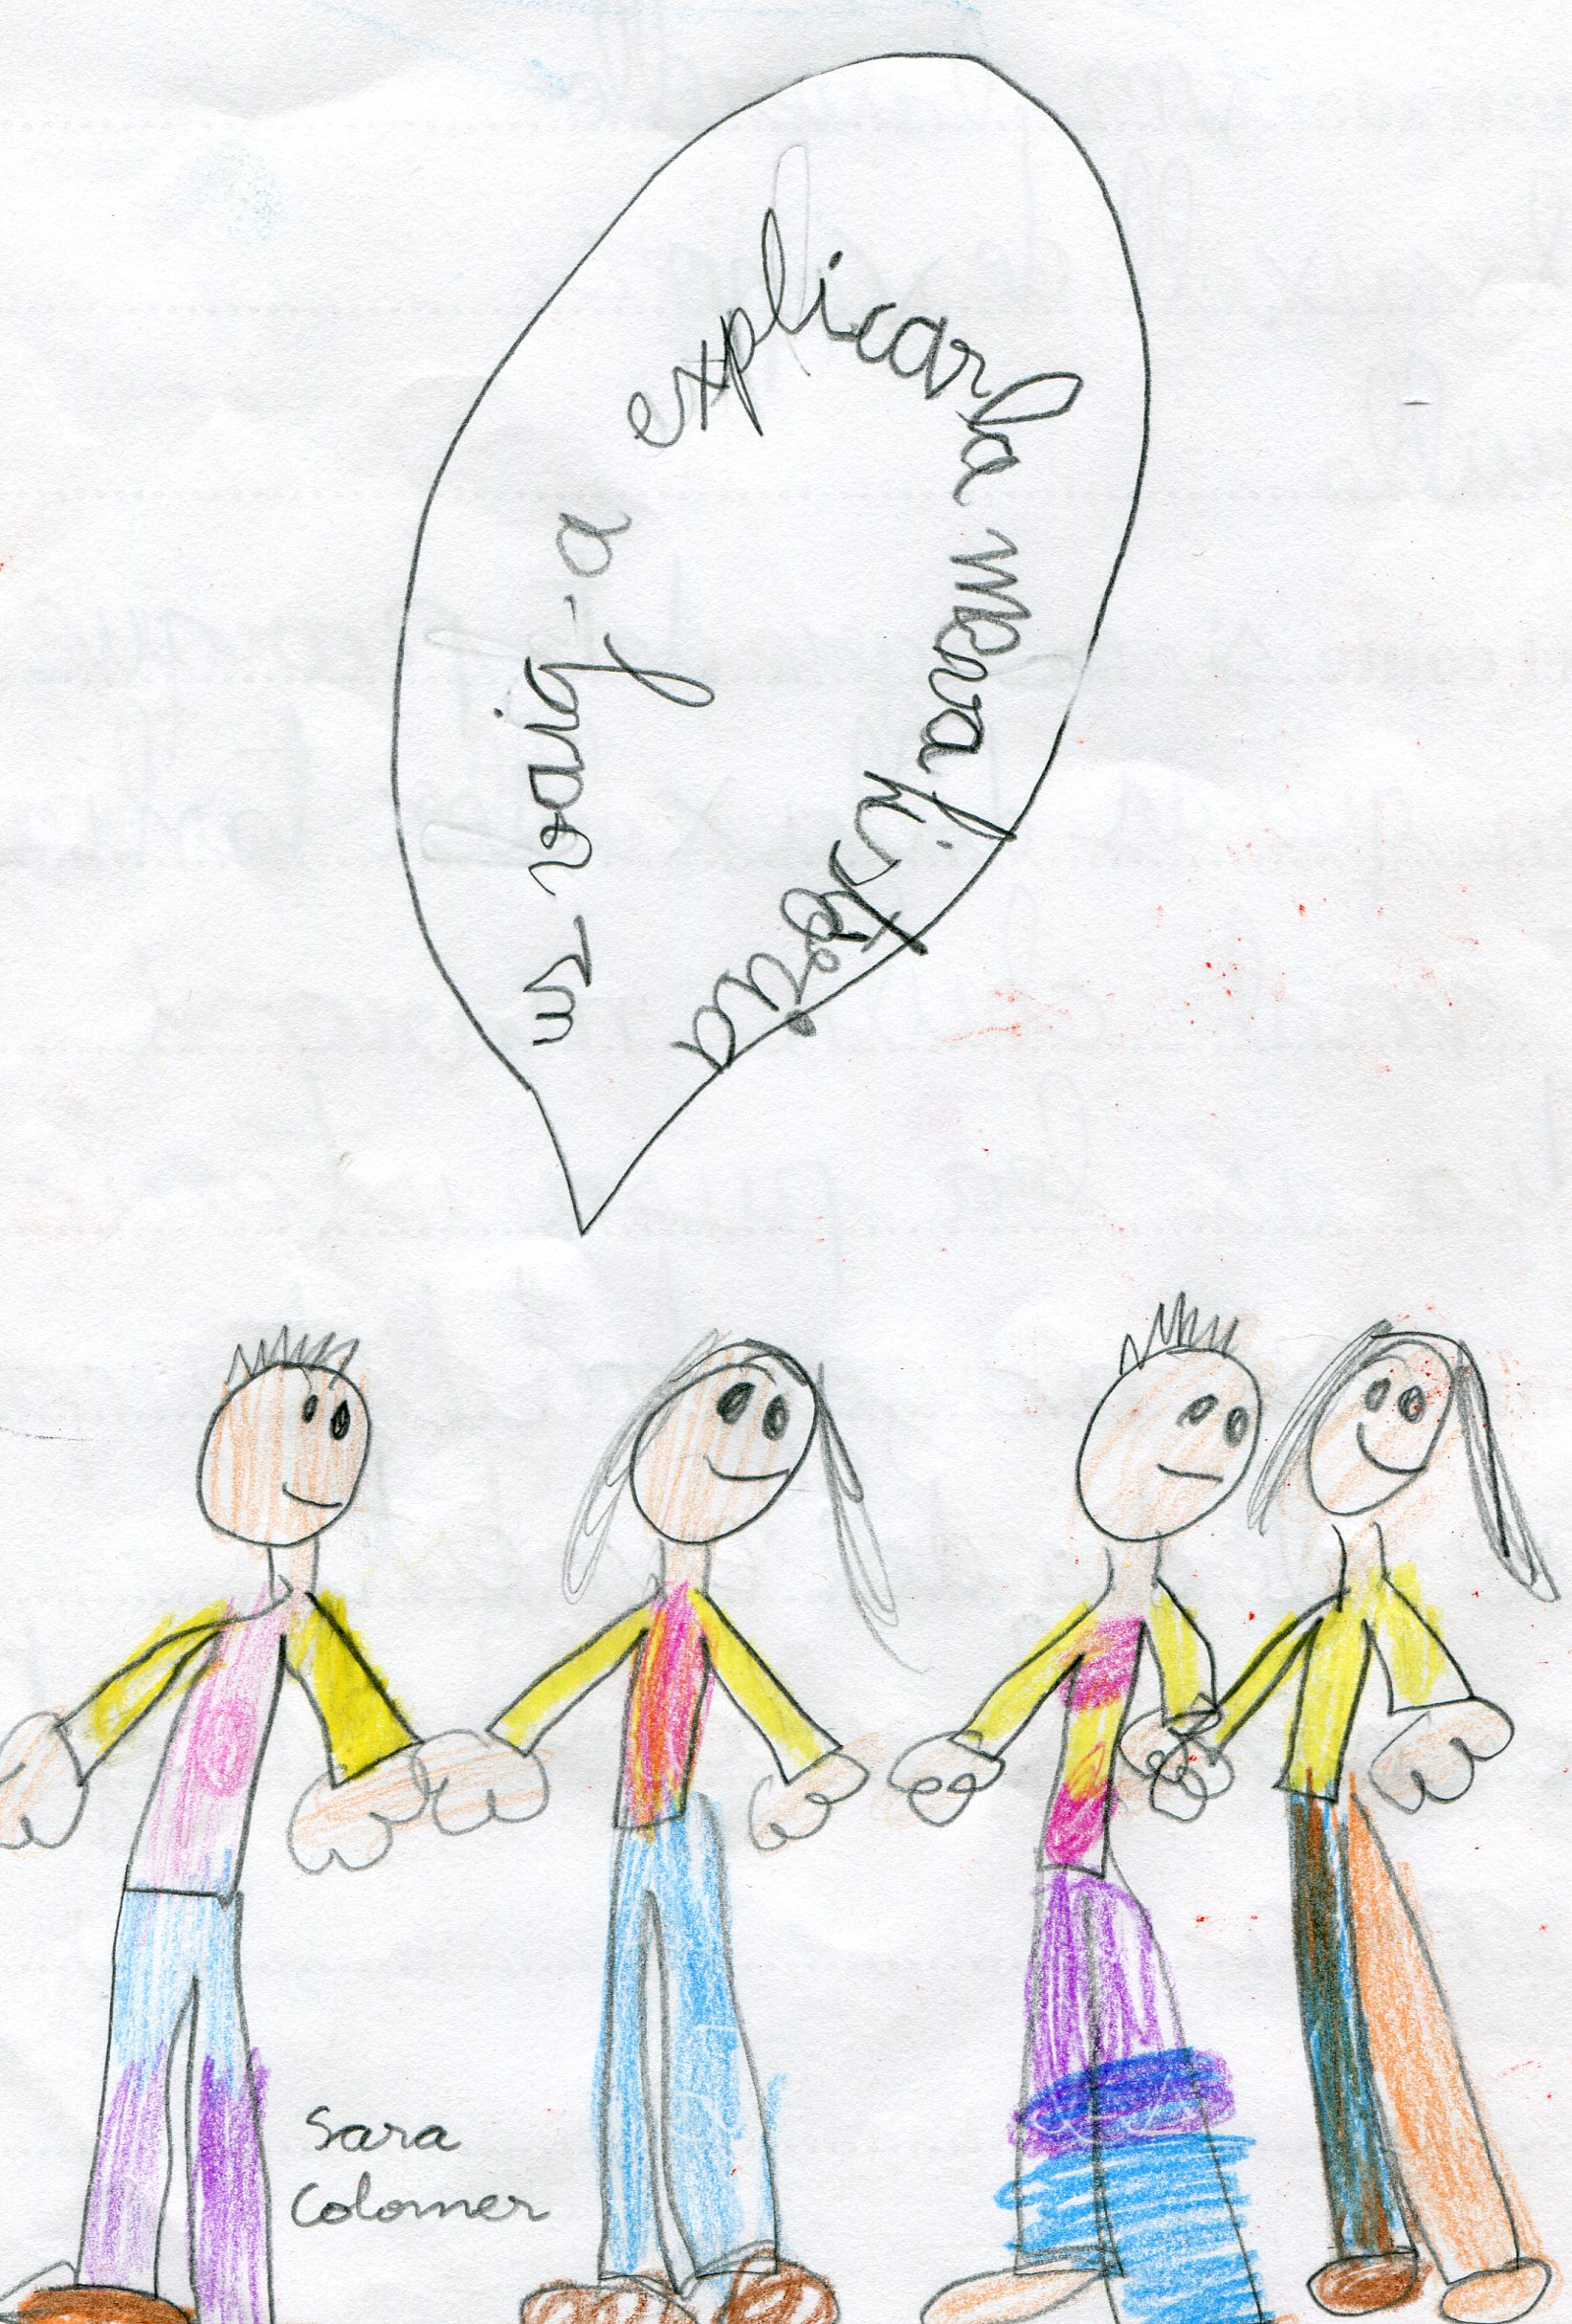
\includegraphics[width=5cm,keepaspectratio]{fem_escola/img/ressenya_img007.jpg}}

Un nen que es diu Xavier tenia un gat marró molt “xulo”, però un dia es va posar histèric.

M’ha agradat aquest conte perquè el dia de l’aniversari de l’Ernest, en Xavier li regala un gat. 

\authorandplace{Sara Colomer}{2n de Primària}


\subsection*{Feu-me cas!}
\emph{Autor: Anke de Vries     Editorial: Cruïlla}

En Kees no estimava el seu germà, en Ron, i la seva mare li va portar un regal que era una pilota i en Kees va estimar el seu germà.

M’ha agradat perquè han fet els dibuixos molt bé.

\authorandplace{Èric Ramos}{ 2n de Primària}

\subsection*{El vell mariner}
\emph{Autor: Geronimo Stilton  Editorial: Destino}

\noindent\fbox{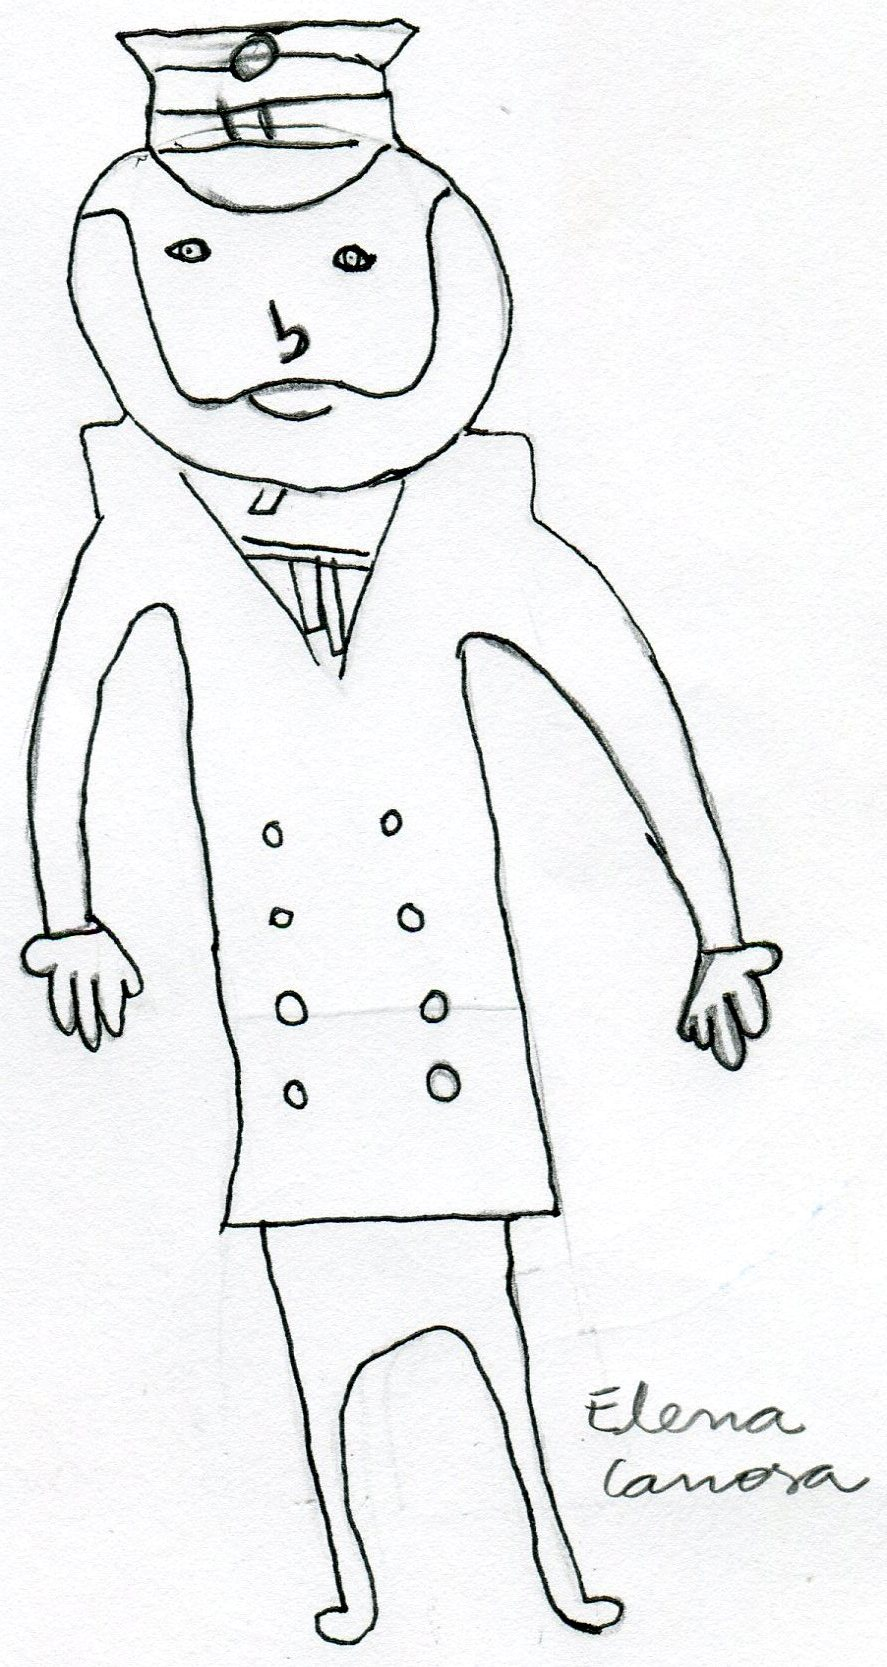
\includegraphics[width=5cm,keepaspectratio]{fem_escola/img/ressenya_img008.jpg}}

Aquest llibre tracta d’un mariner que un dia va a pescar i pesca una sirena.  Se l’emporta a casa seva i li recorda una senyora que anava amb cadira de rodes....

M’ha agradat molt perquè m’agraden els vaixells

\authorandplace{Elena Canosa i Damià Rubio}{3r de Primària}


\subsection*{Llegeix-me si us plau!}
\emph{Autor: Frank Sales.  Editorial: Cruïlla}

\noindent\fbox{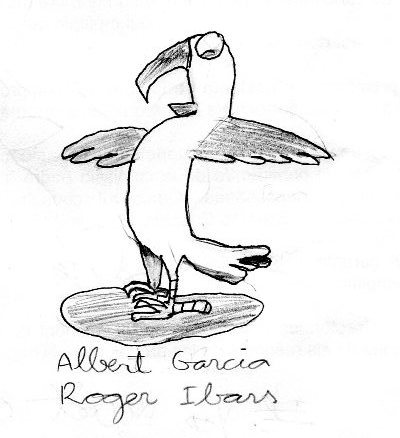
\includegraphics[width=5cm,keepaspectratio]{fem_escola/img/ressenya_img006.jpg}}

Aquesta història parla d’un llibre en un prestatge d’una biblioteca. Aquest llibre té màgia: les lletres parlen! Demanen a la gent que llegeixin perquè no se’ls emportin de la biblioteca. Un dia el llibre cau a sobre de la Laia i comença llegir el conte del lloro Pepet.

M’ha agradat perquè el lloro Pepet comptava d’una manera molt estranya.

\authorandplace{Albert Garcia i Roger Ibars}{ 3r de Primària}


\subsection*{Las aventuras de Ulises}
\emph{Autor: Geronimo Stilton    Editorial: Destino.}

Geronimo Stilton va a una illa, allà troba uns ratolins molt rics i els agrada fer aventures. Entre aquests hi ha el gran capità que no para de parlar d’ Ulisses, que si domina el mar, que si és molt poderós,... Aleshores, Geronimo Stilton va junt amb el capità en un vaixell. De sobte, l’Ulisses neda fins on és el vaixell i amb el seu poder els el trenca. Aquells van en busca de l’Ulisses,... 
	
Aquest llibre m’ha agradat molt per les aventures.

\authorandplace{Axel Santos}{4t de Primària}

\subsection*{Els casos de l’inspector Formiga}
\emph{Autor: Joan de Déu Prats    Editorial: Marge}

\noindent\fbox{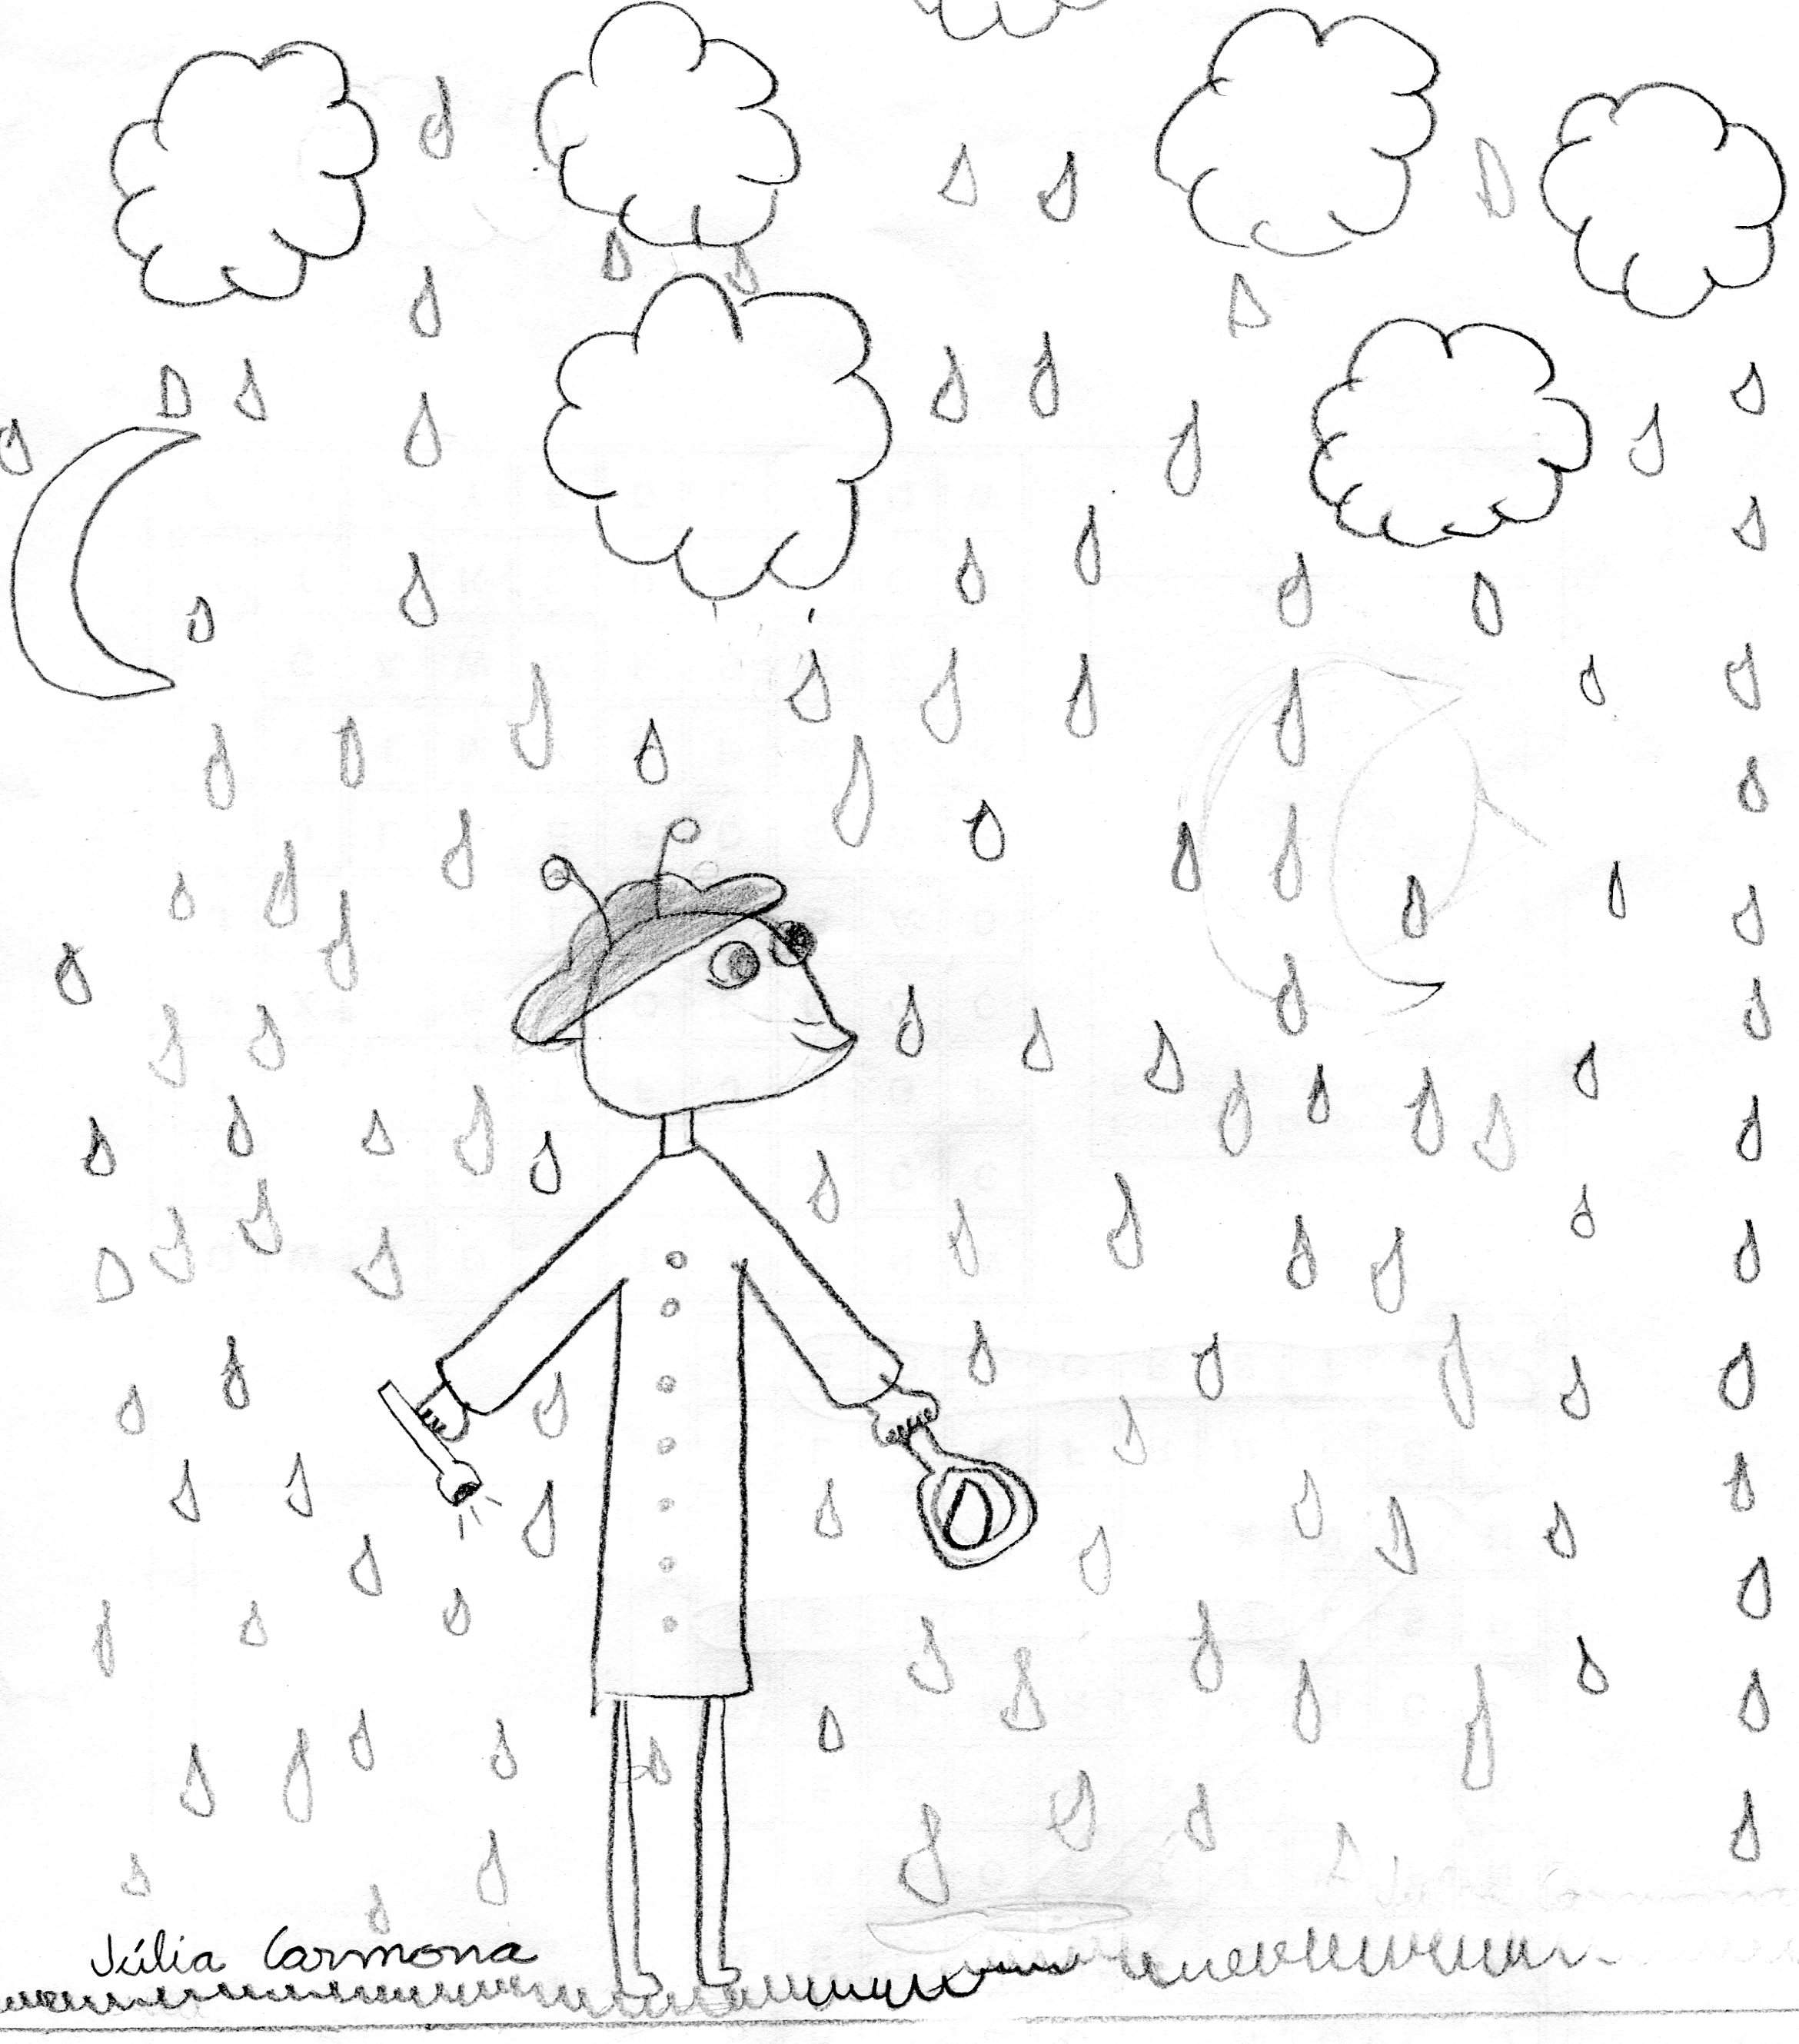
\includegraphics[width=5cm,keepaspectratio]{fem_escola/img/ressenya_img003.jpg}}

És una formiga inspectora que resol casos dels insectes que són assassinats i dels desapareguts. El cas és d’un escarabat que se’l troba mort al carrer i comença a investigar; troba petjades, un ganivet,...

A mi aquest llibre m’ha agradat perquè va d’espionatge i de misteri. El recomano als alumnes de Primària.

\authorandplace{Júlia Carmona}{ 4t de Primària}

\subsection*{Arcanus}
\emph{Autor: Care Santos   Editorial: Planeta}

La història d’aquest llibre ens parla de nens que tenen uns dons especials i que han de cooperar entre ells per salvar el món del malvat Maghul. Aquest llibre forma part d’una col·lecció de dotze títols. A cada un es presenta un dels nens i , a més a més, hi surten bèsties com per exemple un Fènix o un Hipògrif. 

A mi m’ha agradat molt. Us el recomano.

\authorandplace{Oriol Fossas}{ 5è de primària}

\subsection*{Escombres voladores}
\emph{Autor: Ann Jungman    Editorial: Vicens Vives}

Aquest llibre tracta de tres bruixes que a les nits de lluna plena fan encanteris dolents. Dues de les bruixes decideixen no tornar a fer mai més de bruixa. La bruixa que queda s’enfada amb les altres i les insulta. Al cap d’un temps una de les bruixes demana ajuda a les altres. L’ajuden encara que les hagués tractat de mala manera. Finalment la bruixa que no s’havia portat bé es casa gràcies a les seves companyes.

\authorandplace{Carla Salas}{5è de Primària}

\subsection*{T’escriuré}
\emph{Autor: Glòria Llobet.   Editorial: Baula}

L’Anna vivia a Gandia (València). Allà va tenir moltes amistats, especialment  un noi,en Guillem. Un dia els seus pares li comuniquen que se n’han d’anar a viure a Manlleu (Barcelona). Allà haurà de fer noves amistats i superar la seva tristesa.

Aquest llibre m’agrada perquè aquesta noia ha d’anar passant “obstacles” en la seva vida i no saps com reaccionarà. També perquè es una història d’amistat i de comèdia.  

\authorandplace{Marc Luna}{6è de Primària}

\subsection*{Mutació fatal}
\emph{Autor: R.L.Stine  Editorial: Edicions primera plana S.A.}


\noindent\fbox{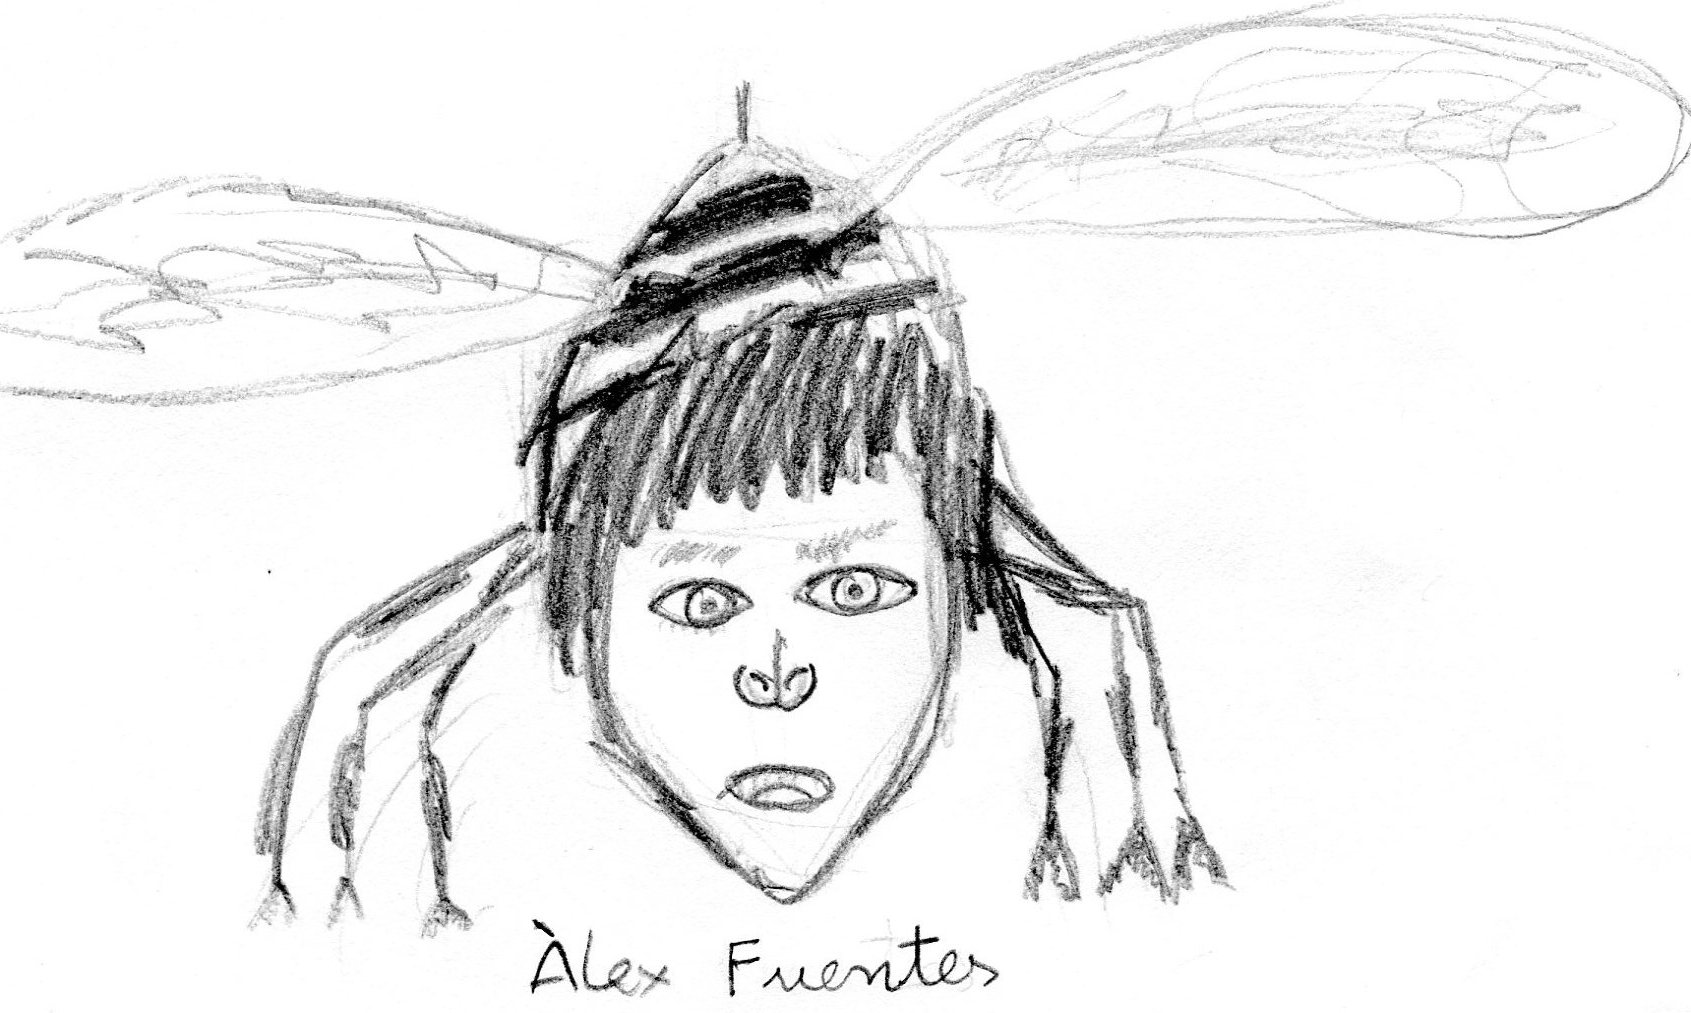
\includegraphics[width=5cm,keepaspectratio]{fem_escola/img/ressenya_img005.jpg}}

Gary Lutz és un nen que no suporta la seva vida, té por de les abelles i se seny empipat per tothom, fins i tot la seva germana es posa amb ell. El senyor Andretti, el seu veí, té un rusc d’abelles. Al nen li fan por les abelles i el senyor Andretti li fa bromes amb les abelles perquè les controla. Un dia ,el nen rep un paper d’una empresa que tenia una màquina que podia canviar les vides en un temps determinat. El nen no s’ho pensa dues vegades i va a l’edifici de l’empresa. A l’edifici, degut a una infiltració d’una abella, Gary Lutz es convertirà en l’insecte que menys li agrada.


\authorandplace{Àlex Fuentes}{6è de Primària}



\subsection*{Lior}
\emph{Autor; Pradas, Núria. Ed.}
 
Us recomano aquest llibre perquè és molt entretingut. Parla d’un món del futur on no hi ha sentiments ni llibertat, només val l’esport i la competició. En Lior descobrirà que hi ha altres habitants d’aquesta societat que pensen de forma diferent i lluitarà per aconseguir un món diferent.

\authorandplace{Joan Colldecarrera}{1r ESO}


\subsection*{Cartas de invierno}

\emph{Autor; 	Fernández Paz, Agustín. Ed.SM}

El pintor Adrián Novoa, aconsejado por su amigo Xavier, compra una casa en una aldea de Galicia. Es la casa de sus sueños. En ella quiere encontrar la paz necessaria para encontrar nueva inspiración en su pintura. Pero la casa esconde un profundo y oscuro misterio que atrapa a Novoa como un imán.

Recomiendo este libro porque te engancha desde el principio, es decir, no puedes parar de leer, porque cada vez que acabas un capítulo quieres leer el siguiente. És un libro de misterio y algo de terror.

\authorandplace{Sergi Cervera}{1r d’ESO}



\subsection*{Fi de curs a Bucarest}
\emph{Autor; Pinyol, Joan. Ed. Baula}

Radu Petrescu és un noi que ha de marxar de casa perquè el seu pare l’ha obligat a robar i el persegueix la policia.

Radu se’n va de Cosbuc, el seu poble, cap a Bucarest, la capital de Romania.

Durant el viatge cap a Bucarest coneix  uns nois ( Vasile, Moisei ,l'Ovidi i en Juliu) que pertanyen a una organització que no vol permetre que Romania entri a La Unió Europea. En Radu s’uneix a ells ja que no té diners.

Un grup  d‘estudiants catalans arriba a Bucarest de viatge de fi de curs de 4t   d’ESO, entre ells un noi anomenat Raül. 

El dia de l’arribada dels catalans el grup d’en Radu i d’en Raül es troben en  un parc  i es barallen. Durant aquest enfrontament els amics d’en Radu li roben la càmera a en Raül.

En Raül havia de recuperar la càmera fos com fos, ja que era del seu pare.  

En Radu li promet que  l’ajudarà a recuperar la càmera. Uns dies més tard en Radu desapareix.

En Raül i la Tatiana, una amiga romanesa, presenten una denúncia per la desaparició d’en Radu Petrescu. ...

 I la història continua..............

\authorandplace{Carla Jiménez}{2n ESO}

\subsection*{Sis històries al voltant d’en Màrius}
\emph{Autor: Sierra i Fabra, Jordi. Ed Planeta	}

Aquest llibre tracta de la vida d’un noi, en Màrius, que relata la seva vida des que neix fins als divuit anys; no obstant, ell no n’és el narrador sinó les diferents persones que ens l’expliquen, gent del seu entorn, família i amics.

Cada història és un any o dos de la seva vida, i cada persona explica el que va viure amb en Màrius

Si el llegiu veureu que en Màrius acaba tenint problemes amb les drogues i que no li serà gens fàcil sortir-se’n.

Aquest llibre l’he trobat entranyable i fascinant, és d’aquells que el llegiries més d’una vegada

\authorandplace{Maria Garcia}{ 3r ESO}



\subsection*{Pots comptar els estels?}
\emph{Autor: Lowry, Lois. Ed La Magrana}

Som a l’any 1943 i, per a l’Annemarie , viure a Copenhaguen és una barreja de rutina, d’escassetat de menjar i d’opressió per la presència constant de les tropes nazis.
La seva família ajuda els seus veïns a escapar de Dinamarca quan els nazis comencen a endur-se els jueus, i amaguen l’Ellen, la millor amiga de l’Annemarie, tot i córrer el risc de ser descoberts.

\authorandplace{Davínia W. Vilagrasa}{ 3r d’ESO}

\subsection*{Bitllet d’anada i tornada}

\emph{Autor: Lienas, Gemma. Ed. Estrella Polar}

Bitllet d’anada i tornada és el testimoni d’una noia que pateix anorèxia i és ingressada a l’hospital on coneix a altres noies que tenen el mateix problema. Però la Marta, la protagonista, no vol engreixar-se de cap de les maneres ja que té por de patir bulímia. Allà recorda com era la seva vida, abans d’ingressar a l’hospital, amb la família, amb el Rcky, la seva parella, i amb la seva millor amiga, la Clàudia.
Aquesta novel.la la trobo molt recomanable ja que és una història sobre la realitat de molts joves d’avui en dia, és un llibre que et mentalitza. Crec que l’autora sap com explicar i parlar d’aquest tema tan delicat, ens fa veure que l’anorèxia no és cap broma ni cap diversió. És una malaltia molt greu. 

\authorandplace{Raquel Madrenas}{4t ESO}


\subsection*{Memòries d’Idhum}

\emph{Autora: Gallego, Laura. Ed. Cruïlla}

És un llibre que combina molt bé la història d’amor amb la fantasia i un conjunt d’éssers fantàstics
La trama es du a terme a la terra i a Idhum, un món màgic on un tirà anomenat Ashran és al poder. En Jack, la Victòria i els seus amics, els anomenats “la resistència”,  lluitaran per aconseguir la llibertat de la seva terra i la seva i també pròpia.. Escenaris com boscos que creixen a grans velocitats, deserts mortífers, muntanyes canviants i paisatges gelats on hi viuen gegants..., tot plegat és una explosió de fantasia i màgia
\authorandplace{Esteve Pérez}{4t ESO}

\end{news}
